\chapter{Related Work\label{cha:related_work}}


%\section{Sequence-Based Anomaly Detection in Logs}
There has been a large amount of research and development of new approaches for anomaly detection in logs. %TODO alle Quellen einfuegen.
Approaches can be characterised by the following categories: supervised learning models, unsupervised learning models, statistical models, classical machine learning models and finally deep learning models.
% supervised learning methods
Numerous supervised learning methods were applied to solve the problem of log anomaly detection. Liang et al. \cite{liang2007failure} and Yuan et al. \cite{yuan2006automated} trained a SVM classifier to detect errors. Farshchi et al. \cite{farshchi2015anomaly} adopt a regression-based method to find correlations between an operation's logs and the operation activity's effect on cloud resources. Chen et al \cite{chen2004failure} presented a decision tree learning approach to diagnose failures in large Internet sites. However, these methods have two limitations: they rely on system-specific labeled log data for training and do not provide a general method to cope with ever-changing log data.
% unsupervised learning methods

Additionally, unsupervised learning methods have been proposed. Xu et al. \cite{xu2009detecting} use the Principal Component Analysis method to construct a log count matrix, grouping log events to sessions with the session id which is available for every log event. Lin et al \cite{lin2016log} and \cite{vaarandi2003data} both propose approaches that cluster logs.

% deep learning
The recent remarkable advances of deep learning depict new promising paths for anomaly detection in logs. While LSTMs have been put to use in detecting anomalies in time series generally \cite{malhotra2015long}, they have been used in anomaly detection in logs: Du et al. \cite{du2017deeplog} present DeepLog, which is described in detail in section \ref{sec:deeplog}. Zhang et al. \cite{zhang2016automated} use a LSTM similarly. Even though these approaches yield good results, they are not able to cope with changing log data, since log events have to be transformed into fixed indices.

% nlp based
There are studies that have applied NLP techniques and consider log events as natural language. Bertero et al \cite{bertero2017experience} used Google's word2vec algorithm to obtain word embeddings, exploiting the obtained feature space using standard classifiers, like SVM and Random Forest, to detect anomalies. Zhang et al. \cite{zhang2016automated} additionally to using the LSTM model for time series prediction, apply  TF-IDF weight and consider each log event as a word. Brown et al. \cite{brown2018recurrent} use combine attention based models together with word word embeddings. These approaches do not take into account the contextual information in log sequences.

Very recently, LogRobust, which is described in detail in section \ref{sec:logrobust} and LogAnomaly, described in section \ref{sec:loganomaly}, use pre-trained word embeddings, using an attention-based Bi-LSTM model to learn log sequences.


\section{DeepLog: Anomaly Detection and Diagnosis from System Logs through Deep Learning \label{sec:deeplog}}
Du et al. proposed DeepLog \cite{du2017deeplog}, a prominent example of a model that treats system logs as natural language sequences. An overview of the model is depicted in figure \ref{fig:deeplog}. The first step of the proposed model is like in most of the works in the area: Logs are first pre-processed with a log parser, they separate the constant from the variable part. Log templates are mapped to log keys $k_i$, which are just indices between $0$ to the number of different templates. For each log entry $e_i$, the elapsed time between $e_i$ and $e_{i-1}$ are stored in $\vec{v}_{e_i}$, together with parameter values in a parameter value vector. An LSTM is then trained on the sequences $k_i$ to learn normal system execution paths. Given a window size of $h=3$, a sequence of log keys $\{k_5, k_{11}, k_2, k_{14}, k_{15}\}$ would results in the \textit{input sequence} and \textit{output sequence} for training of $\{k_{5},k_{11},k_{2} \rightarrow k_{14}\}$ and $\{k_{11},k_{2},k_{14} \rightarrow k_{15}\}$. Given these sequences of keys, the system is trained to maximise the probability of having $k_i \in K$ as the next log key value, thus learning the probability distribution $Pr(m_t = k_i | m_{t-h},...,m_{t-1})$, so given a log key sequence of length $h$, outputs a probability distribution of all possible log key values. A log key value is treated as normal, if it's among the top $g$ candidates.
 For the detection stage, new log key entries $e_t$ are parsed into a log key $m_t$ and parameter value vector. Then, the trained model is used, to check if the incoming log key is normal, by sending $w = \{m_{t-h}, ..., m_{t-1}\}$ as input. Additionally, the parameter value vector is checked. If the log entry is labeled being abnormal, the model provides semantic information for users to manually diagnose the anomaly. In order to adapt to changing patterns and log entries, the user has the possibility to mark a detected anomaly as a false positive, thus updating the model.

For verification of the model, the authors deployed an OpenStack experiment to fabricate their own log data. They produce over 1 million log entries, with 7\% being abnormal. The model is able to achieve a precision of 0.96, recall of 1.0 and F1-score of 0.98.

Even though the model can be adjusted after the training phase on a particular dataset is already completed, by manually reporting false positives, thus enabling the system to adapt to changing or new sequences of logs, it is not able to dynamically adapt to changes on the log events themselves. If log data changes on the log event level, re-training of the model is necessary.

\begin{figure}[h]
  \centering
  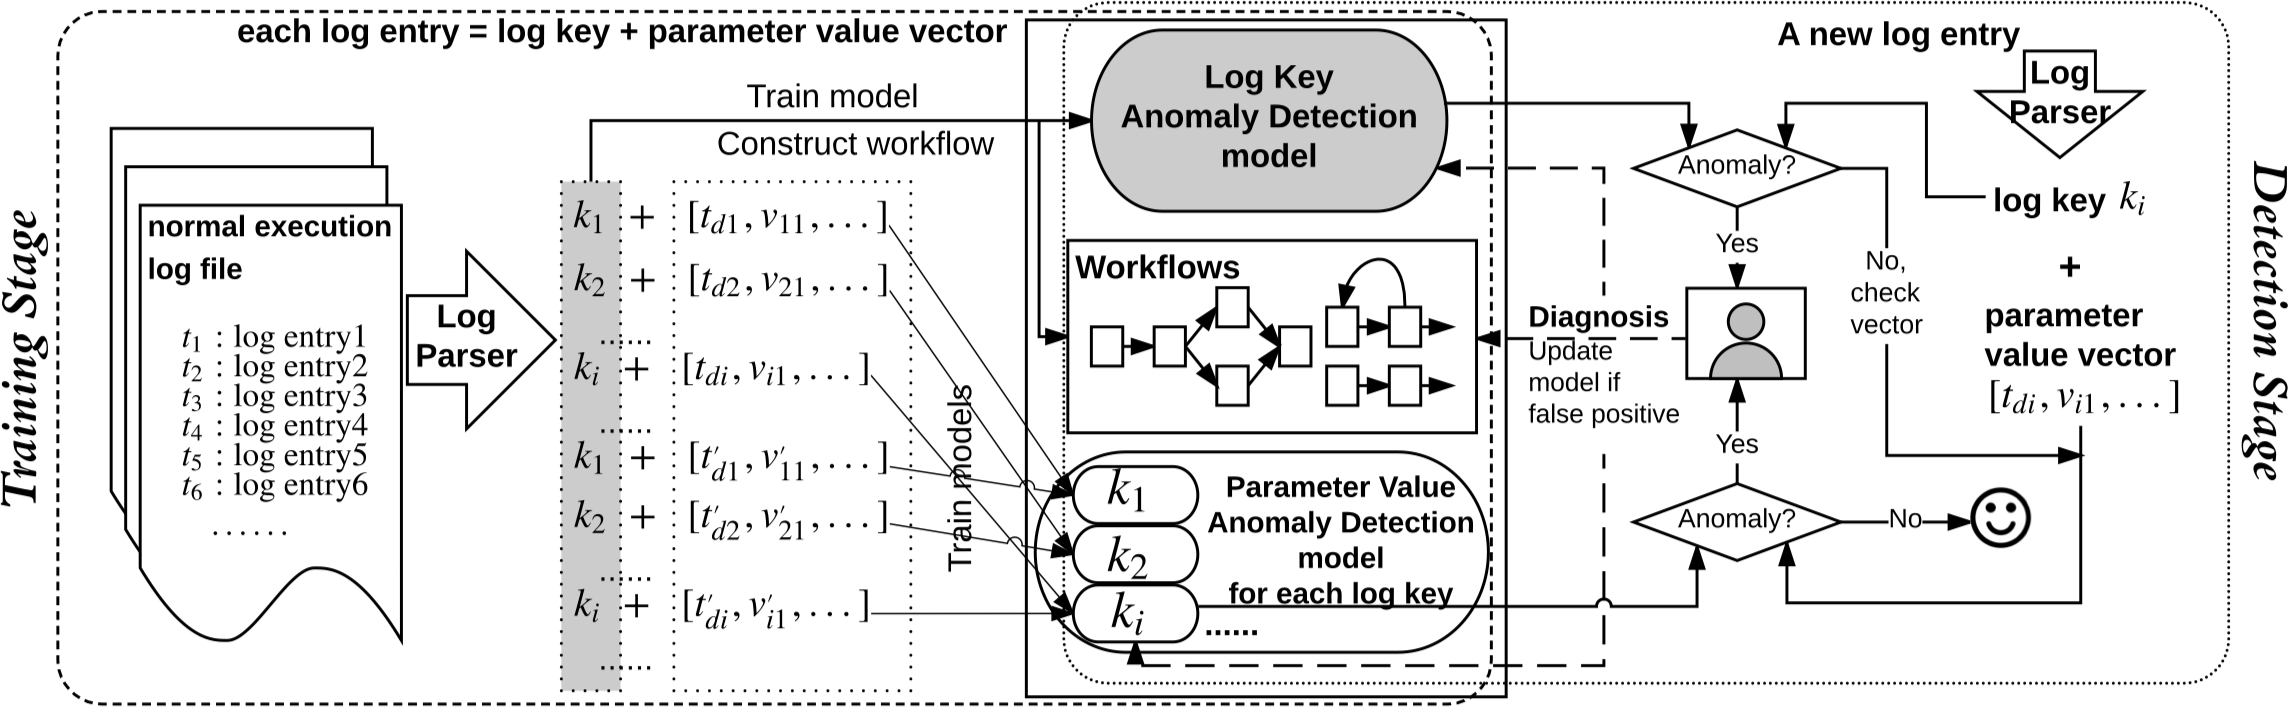
\includegraphics[width=15cm]{deeplog.png}\\
  \caption{DeepLog model overview \cite{graves2013speech}}
  \label{fig:deeplog}
\end{figure}


\section{LogAnomaly: Unsupervised Detection of Sequential and Quantitative Anomalies in Unstructured Logs \label{sec:loganomaly}}
\textit{LogAnomaly}, the approach proposed by Meng et al. \cite{meng2019loganomaly} models a log stream as a natural language sequence. Log event sequences are first parsed into template sequences using FT-Tree. These sequences are then transformed into embedding sequences using a novel word representation method, template2Vec, which is inspired by word2Vec \cite{mikolov2013distributed}. Figure \ref{fig:template2vec} shows the steps included for template2Vec in the offline learning stage: (1) shows the inclusion of common synonyms and antonyms in the English language extracted from WordNet \cite{miller1995wordnet}. Additionally, log-data-specific synonyms and antonyms can be added. In the second (2) step, dLCE \cite{nguyen2016integrating} is used as an embedding model, to generate word vectors that represent the words in templates, which are then transformed (3) into template vectors \cite{meng2019loganomaly}.

After log the sequences of log events $S=(s_1, s_2,...,s_m)$ have been transformed into template vector sequences $V=(v_{s_1}, v_{s_2},...,v_{s_m})$, they apply an Attention-based Bi-LSTM to learn sequences of normal logs. The sequence for detection is a sliding window of the $w$ most recent template vectors, meaning that for a template vector sequence $V_j = v_{(s_j)}, v_{(s_{j+1})}, ..., v_{(s_{j+w-1})}$, the LSTM learns to predict the template vector $v_{j+w}$. Additionally to sequential patterns, LogAnomaly considers quantitative patterns in sequences of templates. For example, opening files should also be closed, so the number of logs indicating that a file was opened should be equal to the number of logs indicating that a file was closed. If a log would break a certain invariant, it can be assumed that an anomaly has occurred during execution. For log messages $s_i \in S_j$, with $S_j$ being a subsequence of $S$, the count vector of the log sequence $s_{i-w+1},s_{i-w+2},...,s_i$ is calculated, denoted as $C_i = (c_i(v_1), c_i(v_2), ..., c_i(v_n))$, with $c_i(v_k)$ being the number of occurrences of $v_k$ in the template vector sequence $v_{i-w+1},s_{i-w+2},...,v_i$. $C_j$, $C_{j+1}, ..., C_{j+w-1}$ are then inputs for the LSTM. This process is laid out in figure \ref{fig:loganomaly} \cite{meng2019loganomaly}.

In order to deal with new log templates in an online fashion, if an arriving log cannot be matches to an existing template, FT-Tree is utilised to extract a template from the new log and its template vector is calculated. Subsequently, the template will be matched on an existing one, based on the similarity among template vectors \cite{meng2019loganomaly}.

For verification of the model, the authors employ a manually labeled BGL dataset containing around 4.7 million logs, and a HDFS dataset with around 11 million logs, both with manual labels on anomalous logs or blocks of logs. For the BGL dataset they achieve a precision of 0.97, recall of 0.94 and F1-score of 0.96. For the HDFS dataset, they achieve a precision of 0.96, recall of 0.94 and F1-score of 0.95 \cite{meng2019loganomaly}.

\begin{figure}[h]
  \centering
  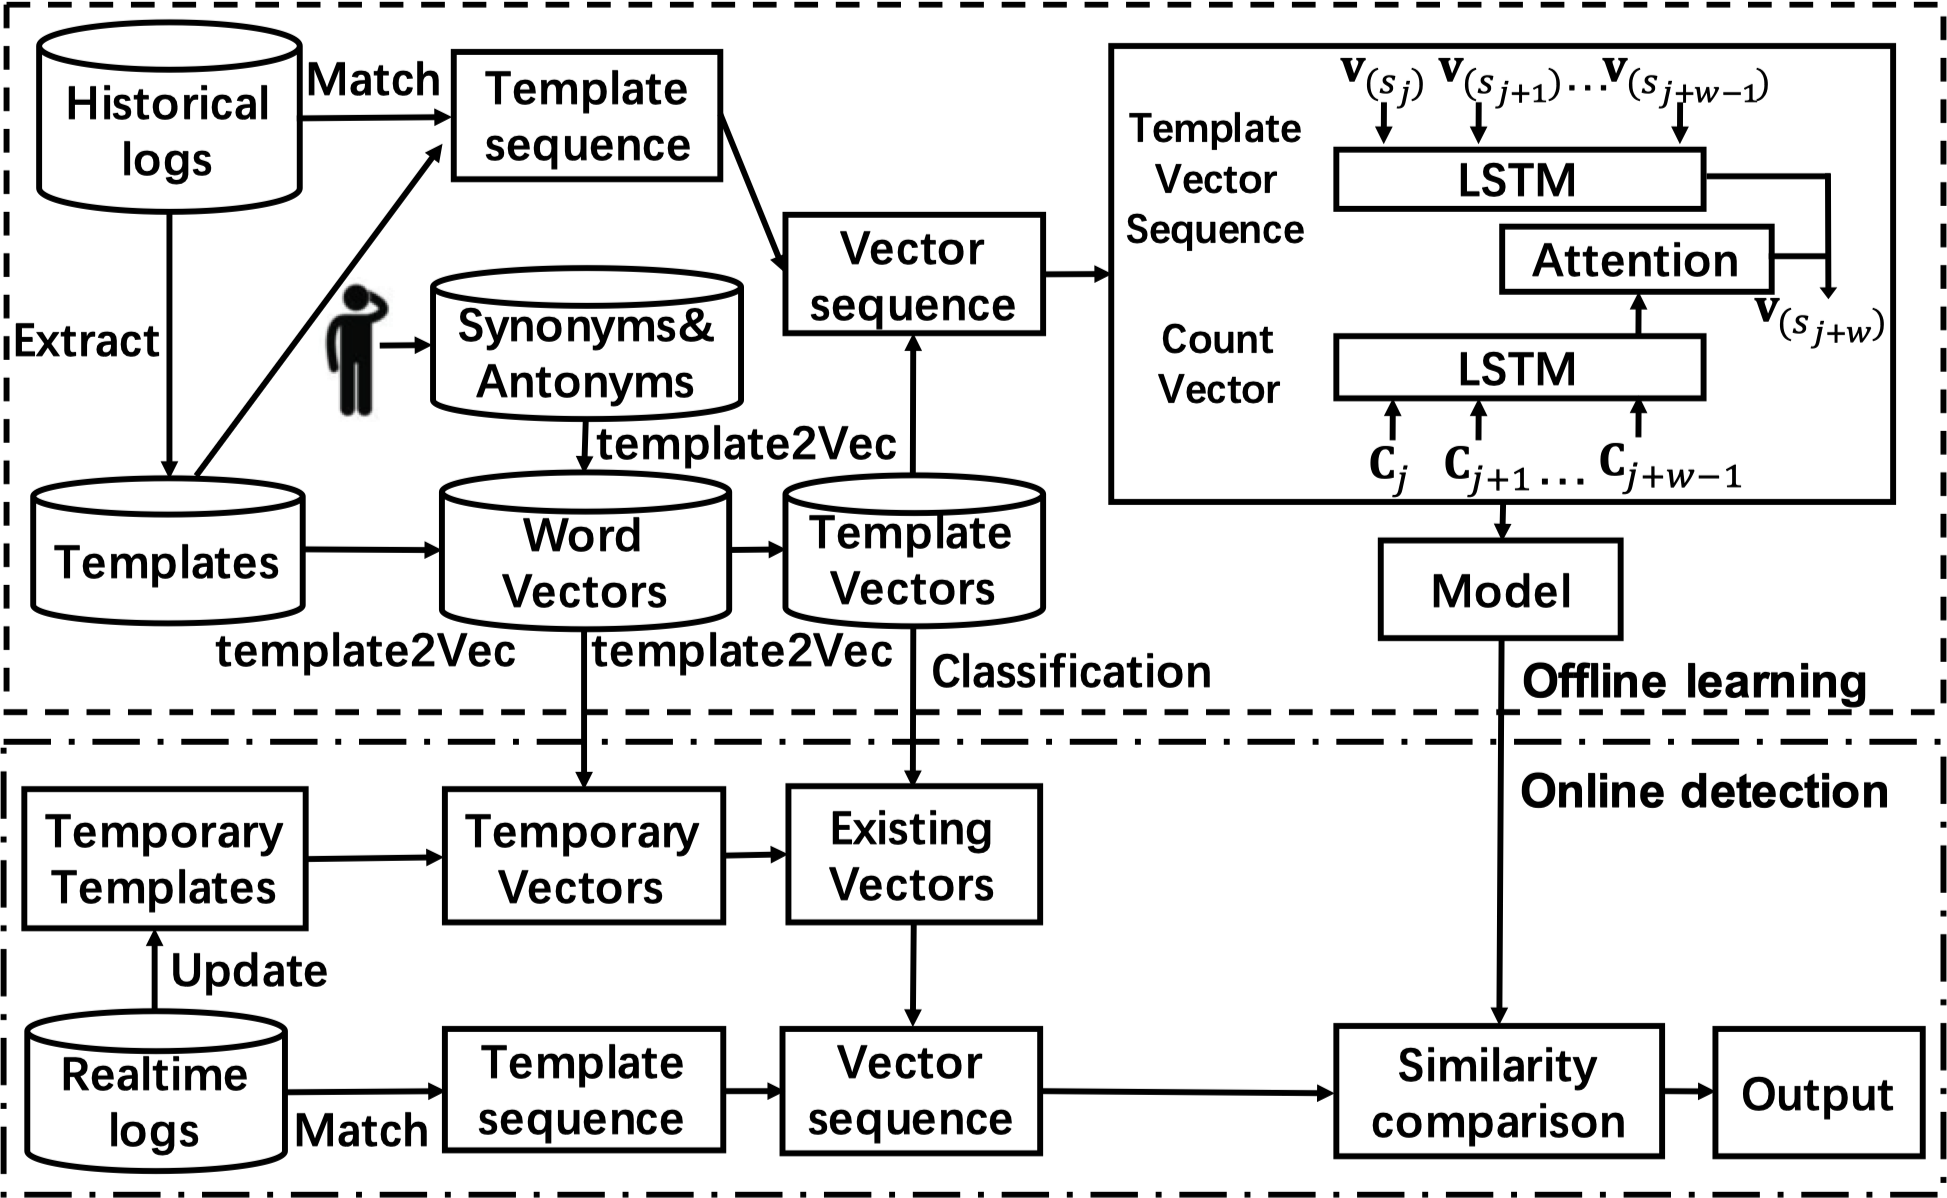
\includegraphics[width=11cm]{LogAnomaly.png}\\
  \caption{LogAnomaly model overview \cite{meng2019loganomaly}.}
  \label{fig:loganomaly}
\end{figure}

\begin{figure}[h]
  \centering
  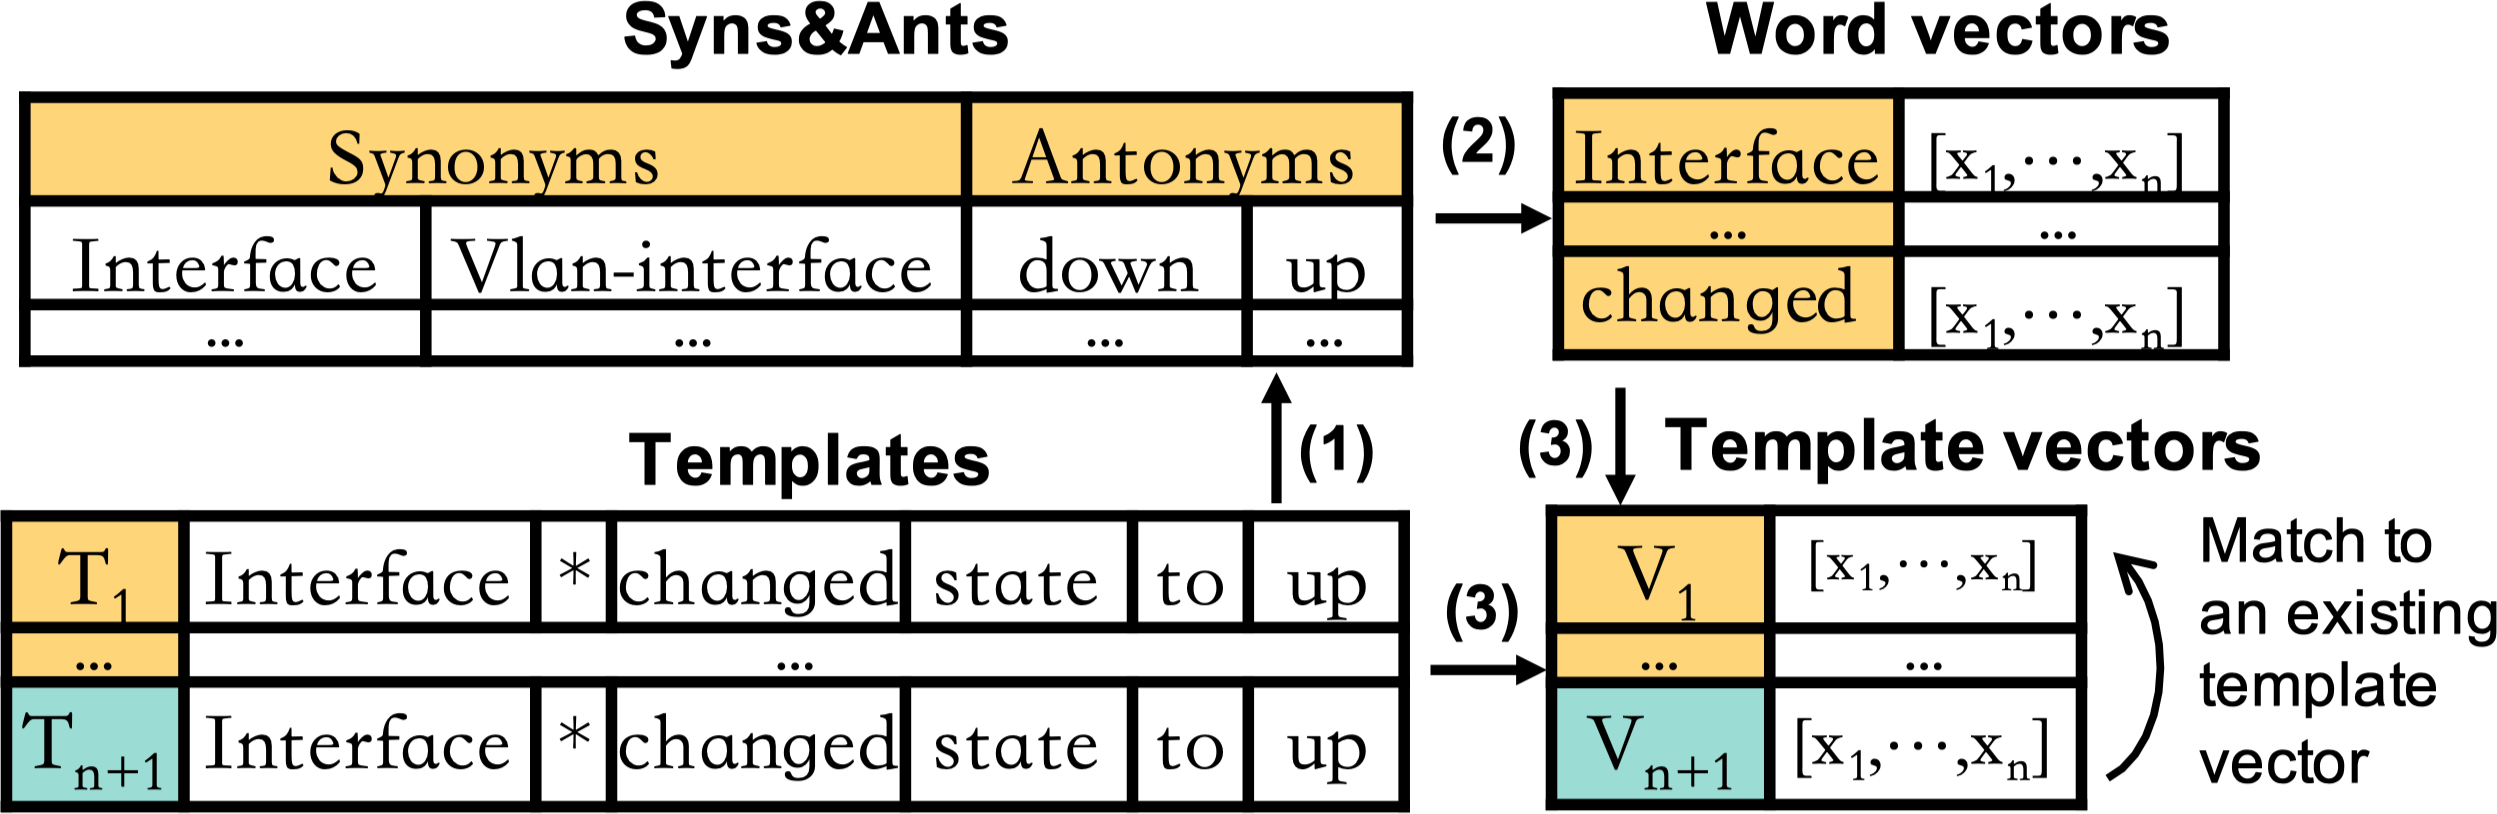
\includegraphics[width=10cm]{templat2vec.png}\\
  \caption{Example of Template2vec \cite{meng2019loganomaly}.}
  \label{fig:template2vec}
\end{figure}


\section{Robust Log-Based Anomaly Detection on Unstable Log Data\label{sec:logrobust}}
Zhang et al. proposed \textit{LogRobust} \cite{zhang2019robust}, emphasising the necessity of anomaly detection on log data being sufficiently robust to the unstable nature of log data which is twofold: They are \textit{evolving}, meaning that frequently modifying source code naturally leads to logging statements getting altered. Also during collection, retrieval and pre-processing of log data, \textit{processing noise} is introduced into the original log data. For example, in large-scale systems, many logs are produced by separate distributed components, potentially leading to missing, duplicated or disordered logs due to network errors or limited system throughput.

In order to capture the semantics of log events, LogRobust treats sequences of log events like sequences of natural language sentences, exactly like in \ref{sec:loganomaly}. After adopting Drain to parse log data and extract log templates from it, they apply FastText \cite{joulin2016fasttext} in order to replace words with corresponding vectors with dimension $d=300$, thus transforming a log-event sentence $S$ into a word vector list $L = (v_1,v_2,...,v_N)$, where $v_i \in \mathbb{R}^d$ and $N$ being the number of tokens in a log-event sentence. Next, all $N$ word vectors that represent a log event are aggregated into a fixed-dimension vector. For this purpose, TF-IDF is applied to measure the importance of words in sentences. For example, if a word appears frequently in a log event, it means that this word is potentially highly representative for this log event, thus increasing its \textit{Term Frequency} (TF) value. On the contrary, if a word appears in many log events, it diminishes the distinguishability of log events, leading to a low \textit{Inverse Document Frequency} (IDF) value. Then, for each word, its TF-IDF weight is calculated by TF $\cdot$ IDF. Finally, the template vector $V \in \mathbb{R}^d$ is obtained by summing up the weighted word vectors.

The log sequences are then split into subsequences and then used as input for an Attention-based Bi-LSTM. Hidden states at time step $t$ of the forward ($f$) and backward ($b$) pass are concatenated as $h_t =$ concat$(h_t^f, h_t^b)$. Log data noise can be reduced with the help of the attention layer, which can automatically learn the importance $\alpha_t$ of a log event, which can be computed by using the weight $W_t^\alpha$ of the attention layer at time step $t$ as follows: $\alpha_t = \tanh(W^\alpha_t \cdot h_t)$. The sum of all hidden states produces the prediction output: $pred = $ softmax $(W \cdot (\sum_{t=0}^{t=T} \alpha_t \cdot h_t))$.

For evaluation, the authors use a HDFS dataset \cite{xu2009detecting} which contains around 24 million log messages with about 2.9\% labelled anomalies, commonly used for benchmarking. They simulate processing noise by applying various small changes to the order of log sequences (unstable seq.) and the evolution of log events by randomly removing or adding words from log events (unstable event). The resulting datasets can be seen in \ref{tab:manipulated_hdfs_dataset}. For an injection ratio of 5\% on \textit{NewTesting1}, LogRobust has a precision of 1.00, recall of 0.91 and an F1-Score of 0.95. Increasing the injection ratio in 5\% steps decreases the F1-Score by roughly 2 percentage points, while the baseline methods degrade more. The results are similar on \textit{NewTesting2}. On the unmodified HDFS dataset, precision is 0.98, recall 1.00 and F1-Score 0.99.

\begin{figure}[h]
  \centering
  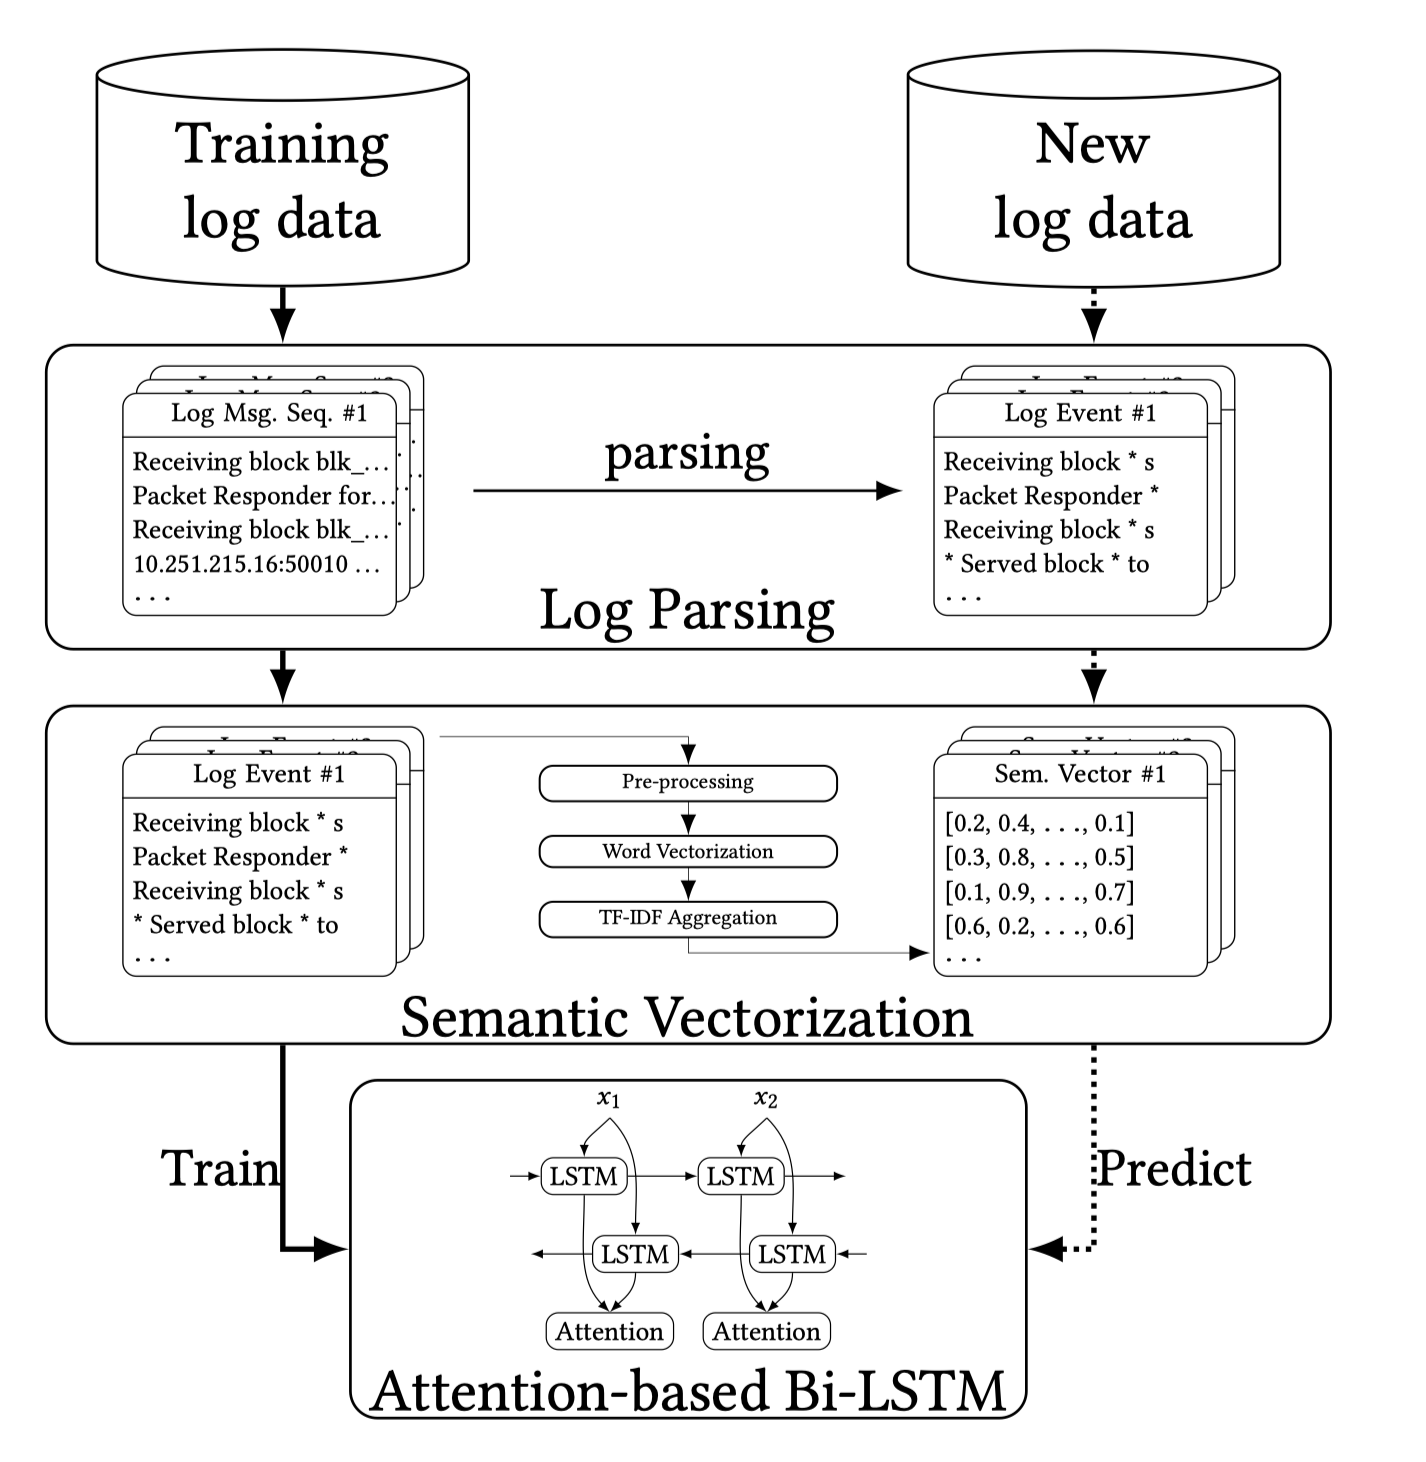
\includegraphics[width=10cm]{LogRobust.png}\\
  \caption{Overview of LogRobust \cite{zhang2019robust}.}
  \label{fig:template2vec}
\end{figure}

\begin{table}[ht]
\centering
\begin{small}
\begin{tabular}{ l c c c c c} 
\toprule
Set & Unstable event & Unstable seq. & Normal & Anomaly & Total \\
\midrule
Training & No & No & 6,000 & 6,000 & 12,000 \\
NewTesting1 & Yes & No & 50,000 & 1,000 & 51,000 \\
NewTesting2 & No & Yes & 50,000 & 1,000 & 51,000 \\

\bottomrule
\end{tabular}
\caption{Manipulated HDFS dataset}
\label{tab:manipulated_hdfs_dataset}
\end{small}
\end{table}









